\documentclass[../main]{subfiles}
\newcommand*\circled[1]{\tikz[baseline=(char.base)]{
            \node[shape=circle,draw,inner sep=1pt] (char) {#1};}}
    \begin{document}
    \setcounter{secnumdepth}{2}
    \chapter{提案手法}
        \section{提案手法の概要}
        本研究は,全天球カメラから取得した画像に基づき通路の特徴を分類する手法を提案する.
        %また,本研究で分類する通路の特徴は先行研究と同様の8種類である.それぞれの図を\fref{figure::new_aisle_type}に示す.\\\\
        %  \circled{1}一本道(straight)\\
        %  \circled{2}行き止まり(dead end)\\
        %  \circled{3}右のみ曲がれる角(right)\\
        %  \circled{4}左のみ曲がれる角(left)\\
        %  \circled{5}十字路(cross)\\
        %  \circled{6}右に曲がれる三叉路(3-way junction\_right)\\
        %  \circled{7}左に曲がれる三叉路(3-way junction\_left)\\
        %  \circled{8}突き当たりの三叉路(3-way junction\_center)
       
        % \vskip\baselineskip
        % \vskip\baselineskip

        本手法の通路分類の流れを\fref{figure::proposed_method}に示す.
        まず,全天球カメラで水平360度の画像データを収集する.次に,YOLOの学習器を用いて画像中の通路やドアなどの物体を検出する.
        通路が検出された場合,通路が検出された方向からどの通路の特徴に相当するかを分類する.
        \fref{figure::proposed_method}の例では,学習器の出力結果から通路が3つ検出されている.また,通路はカメラを取り付けたロボットに対して前,後ろ,
        右方向に検出されている.この通路の特徴から,通路は右に曲がれる三叉路に分類される.
        % %8タイプの通路の画像例
        % \begin{figure}[H]
        %     \centering
        %     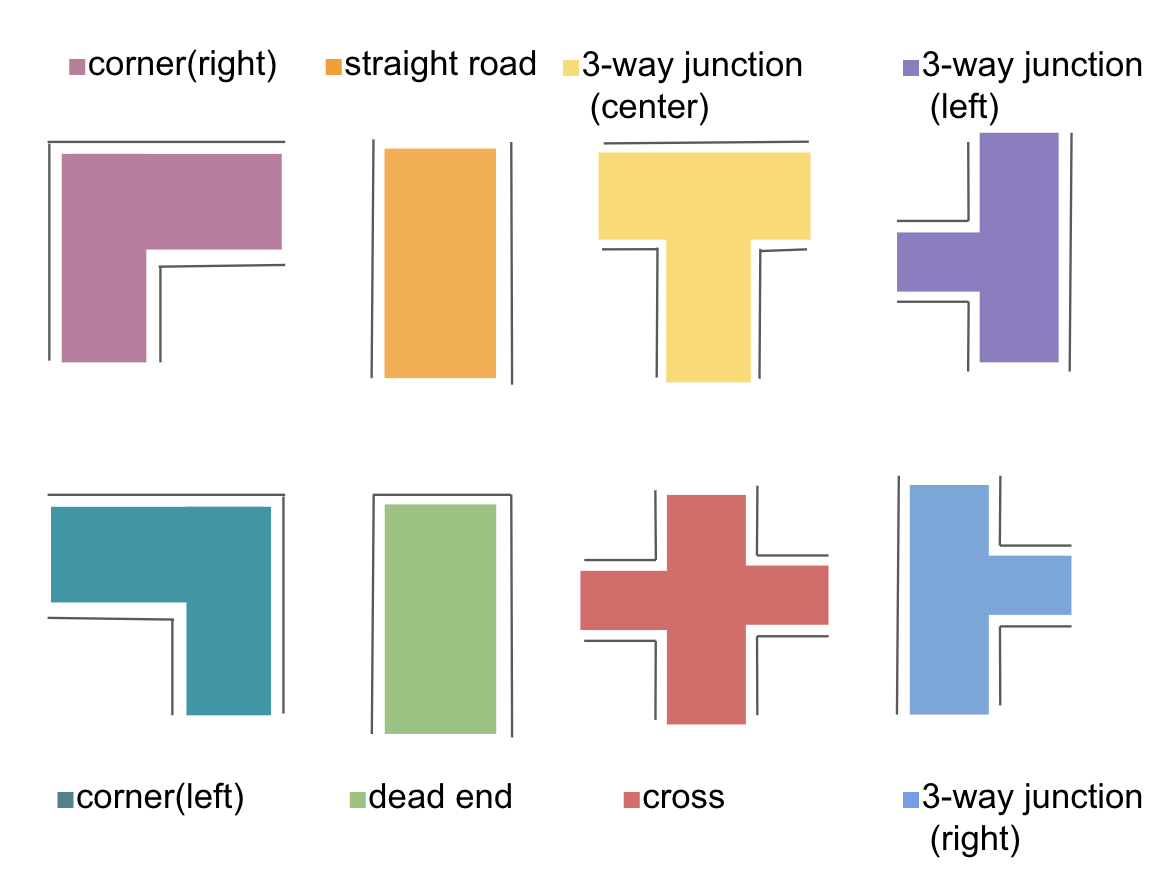
\includegraphics[width=10cm]{../images/aisle_type2.png}
        %     \caption{Type of passage}
        %     \label{figure::new_aisle_type}
        % \end{figure}
        
        %提案手法の簡単な例
        \begin{figure}[H]
            \centering
            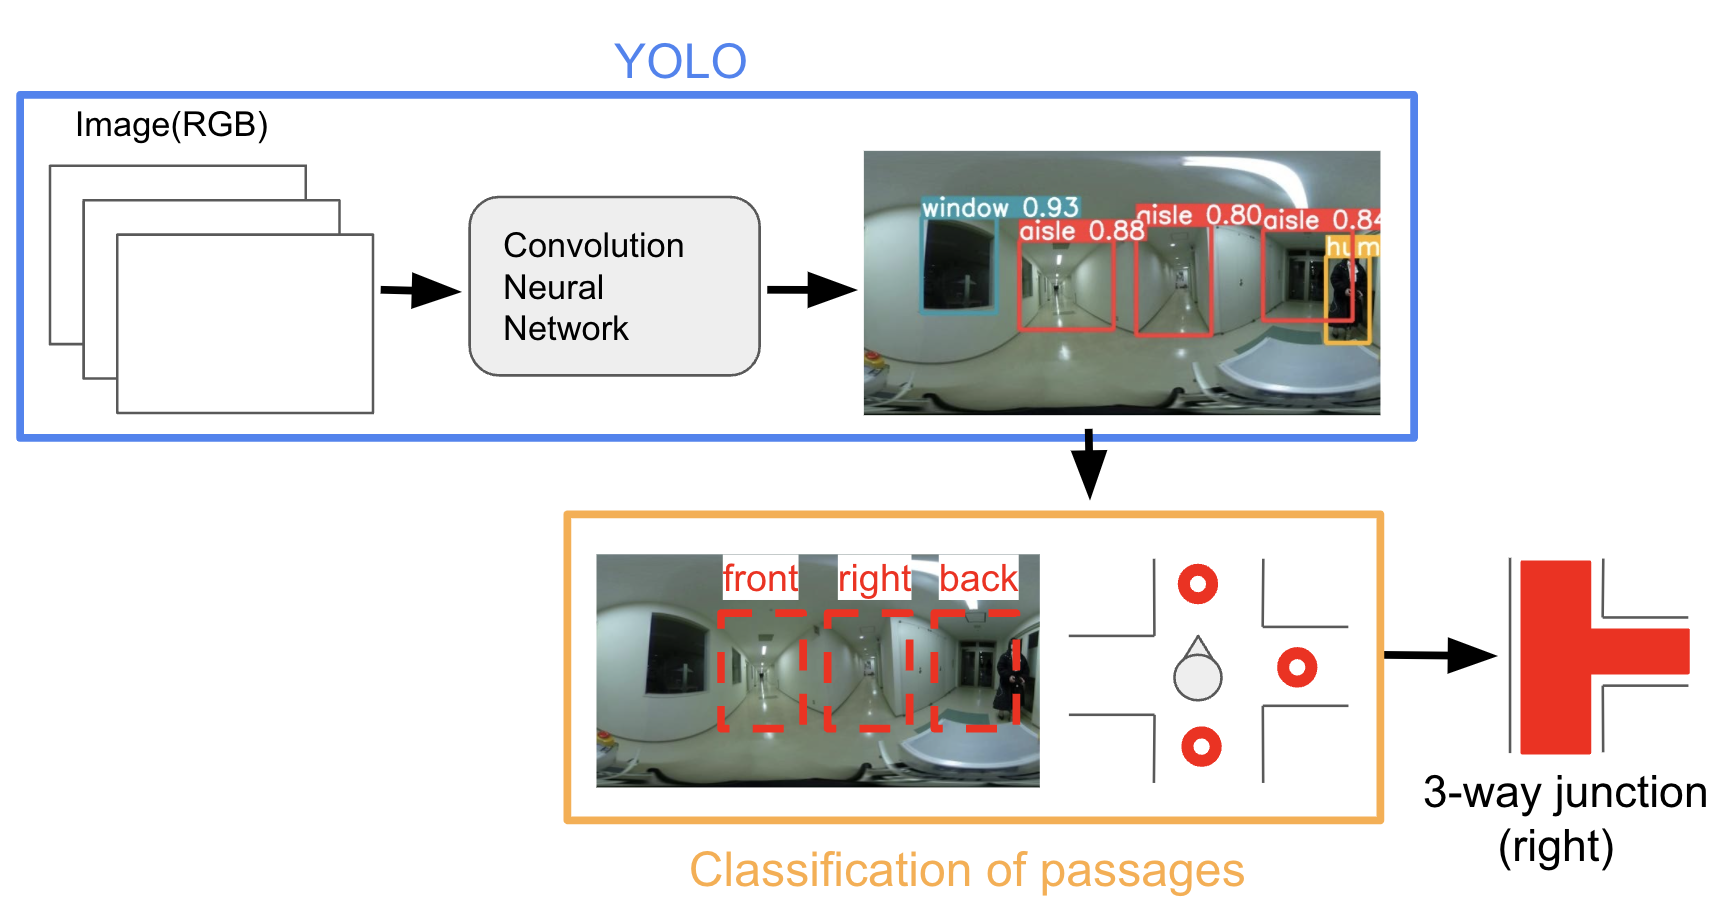
\includegraphics[width=15cm]{../images/proposed_method.png}
            \caption{Flow of passage recognition method}
            \label{figure::proposed_method}
        \end{figure}

        \newpage

        \section{データセットの作成}
        学習モデル作成のため,自作した通路の画像を集めたデータセットを用いて学習を行う.
        学習に用いる画像は千葉工業大学津田沼キャンパス2号館3階の廊下で収集した.
        全天球カメラで取得した画像は通常,\fref{subfigure::no_proc}に示すようにカメラの正面にくる物体が画像の中心に写り,
        後方の物体は画像の左端と右端で分割されてしまう.
        本手法ではカメラの前後左右の各方向にある物体を正しく検出する必要があるため,後方の物体が分割されないようにデータセットの画像に対して
        \fref{subfigure::preproc}に示すような前処理を行う.この処理では,画像の左端1/8を切り取り,右端にスライドさせるという内容の処理を行う.


        データセットは3554枚の画像により構成されており,その一部を\fref{figure::dataset_fig}に示す.
        データセットのラベル付けは11クラスで行い,クラス名を\fref{table::datasets_table}に示す.
    
        %画像の前処理の例
        \begin{figure}[htbp]
          \centering
           \subfigure[no processing image]{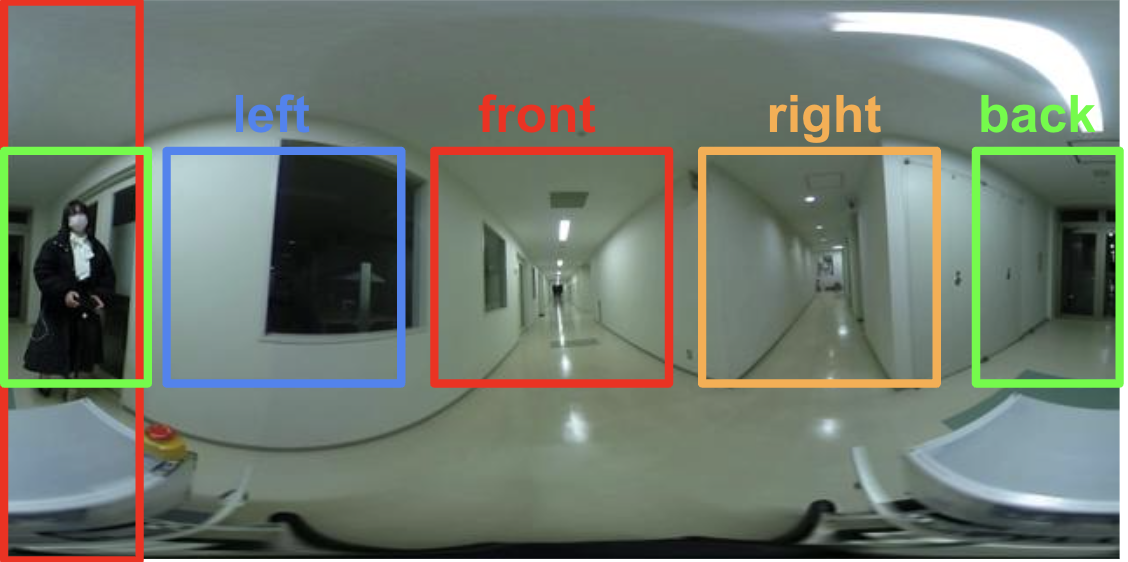
\includegraphics[height=4cm]{../images/no_processing.png}
           \label{subfigure::no_proc}}
           \subfigure[preprocessing image]{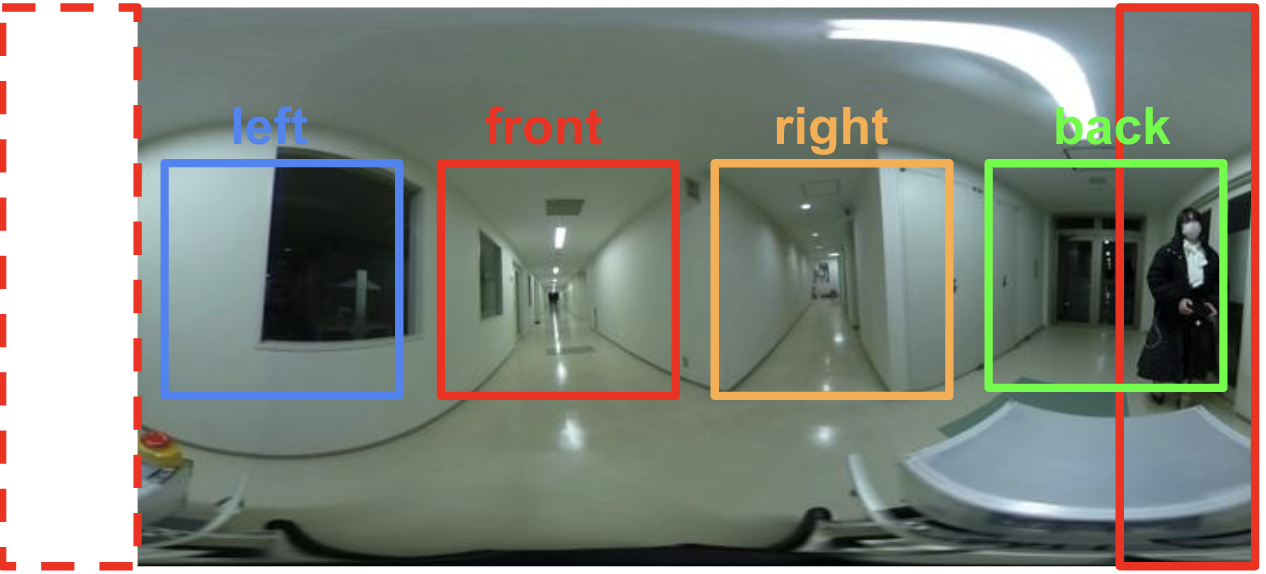
\includegraphics[height=4cm]{../images/after_processing.png}
           \label{subfigure::preproc}}
           \caption{Preprocessing of spherical camera images}
           \label{figure::proc_exp}
        \end{figure}
        
        %自作データセットの画像例
        \begin{figure}[H]
         \centering
         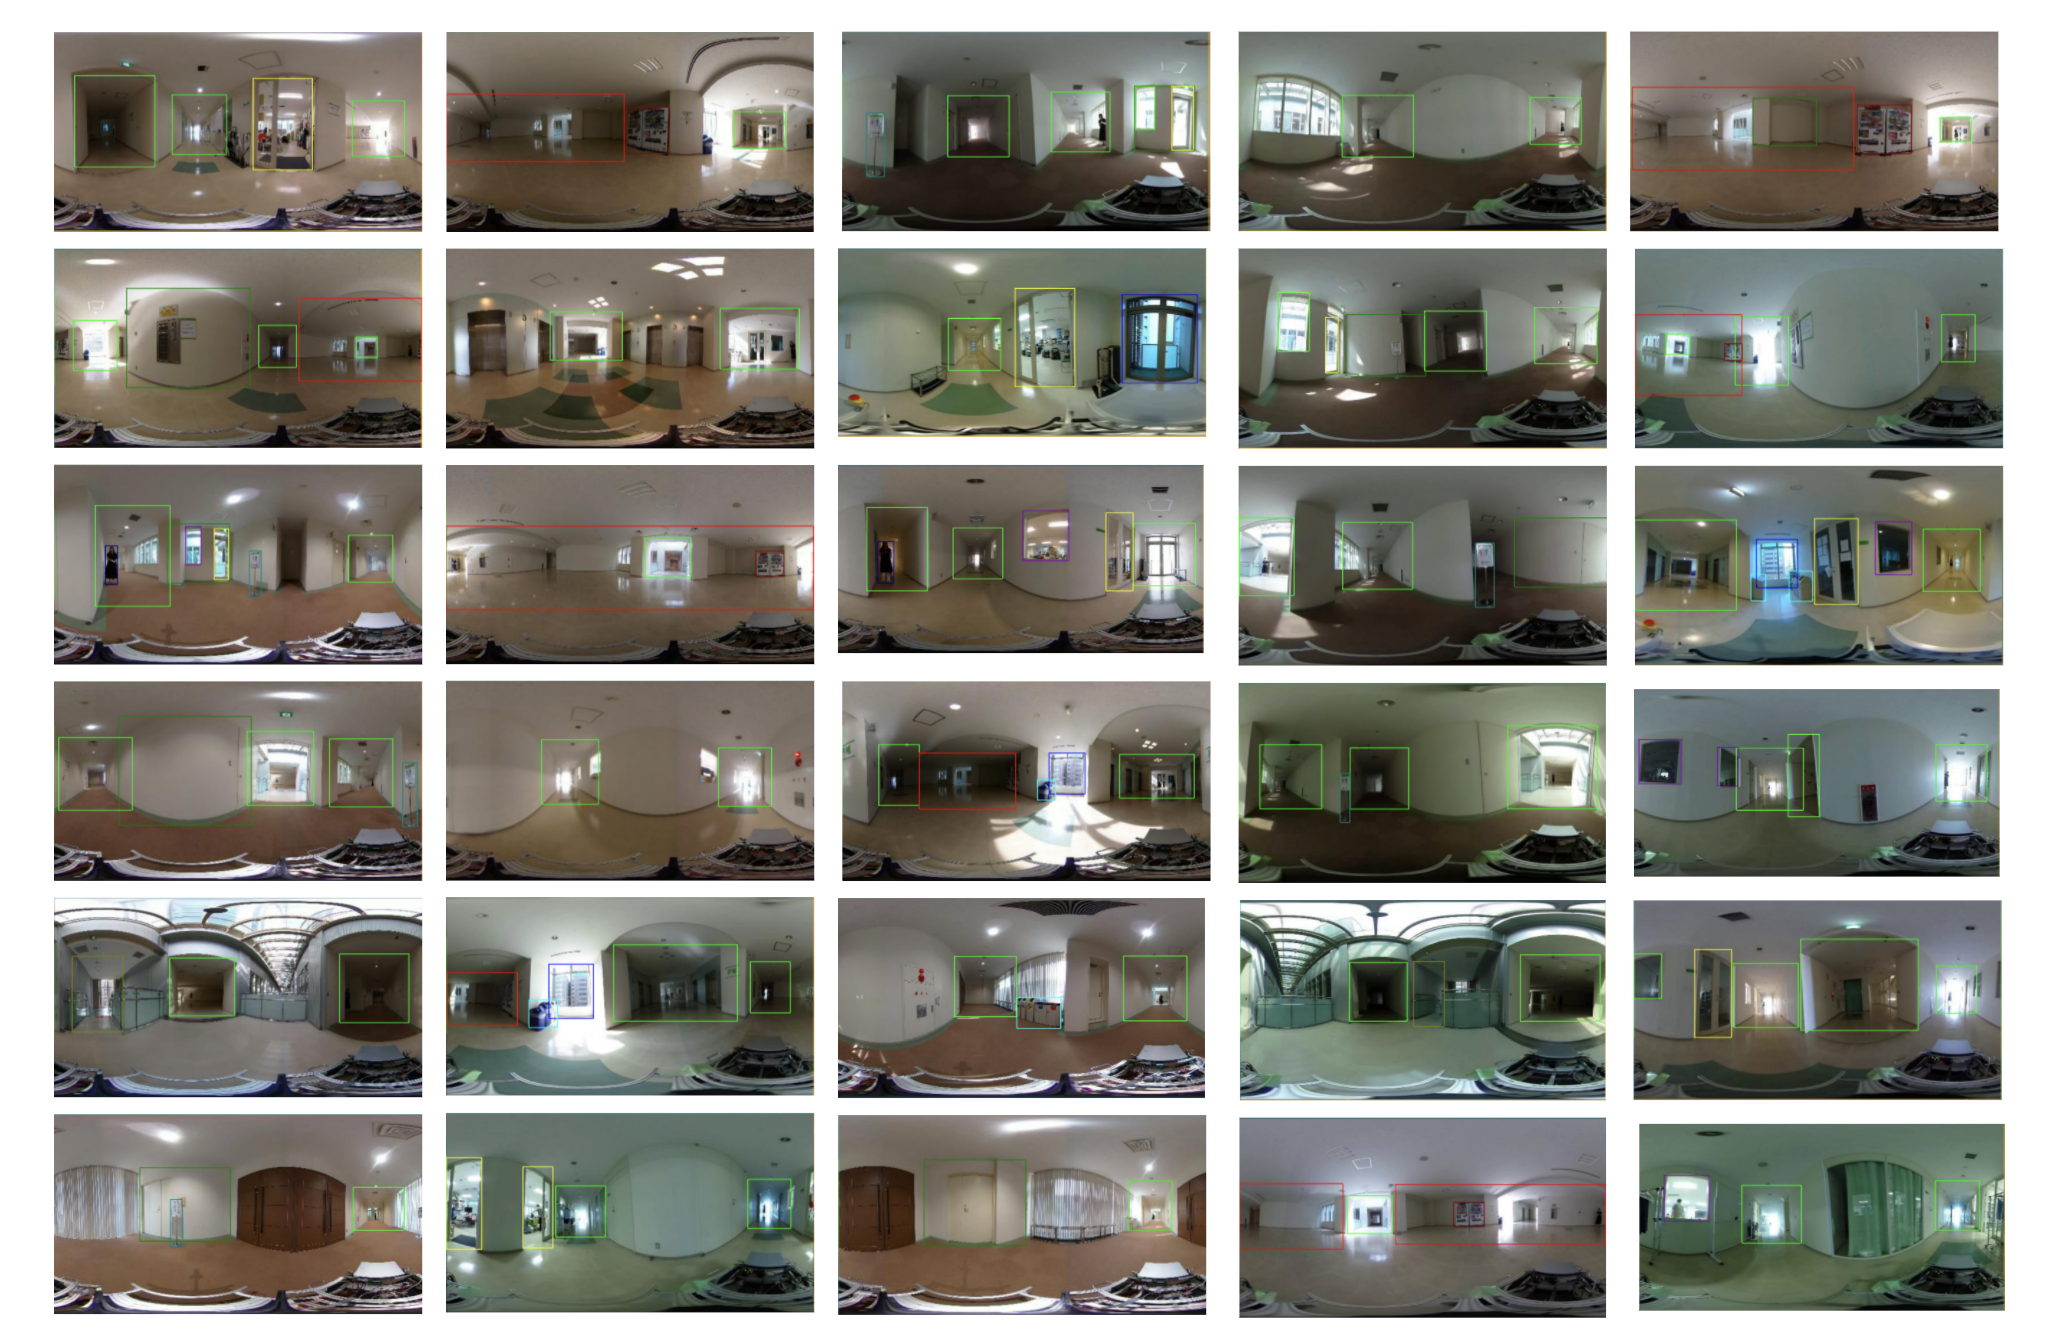
\includegraphics[width=16cm]{../images/dataset_exp.png}
         \caption{An example of a dataset}
         \label{figure::dataset_fig}
        \end{figure}

        %データセットのクラス数
        \begin{table}[H]
            \caption{Class name to be labeled}
            \centering
            \label{table::datasets_table}
            \begin{tabular}{lllll}
            \hline
            name of the class &  &  &  &  \\ 
            \hline \hline
            aisle             &  &  &  &  \\
            end               &  &  &  &  \\
            door\_end         &  &  &  &  \\
            human             &  &  &  &  \\
            door              &  &  &  &  \\
            step              &  &  &  &  \\
            square            &  &  &  &  \\
            vending\_machine  &  &  &  &  \\
            trash\_can        &  &  &  &  \\
            signboard         &  &  &  &  \\
            window            &  &  &  &  \\ 
            \hline
            \end{tabular}
        \end{table}            

        \section{学習の結果}
        作成したデータセットを用いてYOLOv5により学習を行う.トレーニングに用いたネットワークを\fref{figure::}に示す.
        また,学習に用いるデータの構成とハイパーパラメータを\fref{table::learning}に示す.
        

        学習の結果,

        \begin{table}[H]
            \caption{Structure of data used for learning}
            \centering
            \label{table::learning}
            \begin{tabular}{l|l}
            \hline
            \multicolumn{1}{c|}{training}   & \multicolumn{1}{c}{3540}                \\ \hline
            \multicolumn{1}{c|}{validation} & \multicolumn{1}{c}{14}                  \\ \hline
            \multicolumn{1}{c|}{epoch}      & \multicolumn{1}{c}{300}                \\ \hline
            \multicolumn{1}{c|}{batch}      & \multicolumn{1}{c}{8}                   \\ \hline
            \end{tabular}
        \end{table}

\end{document}

%\begin{figure}[H]
        %\centering  
        %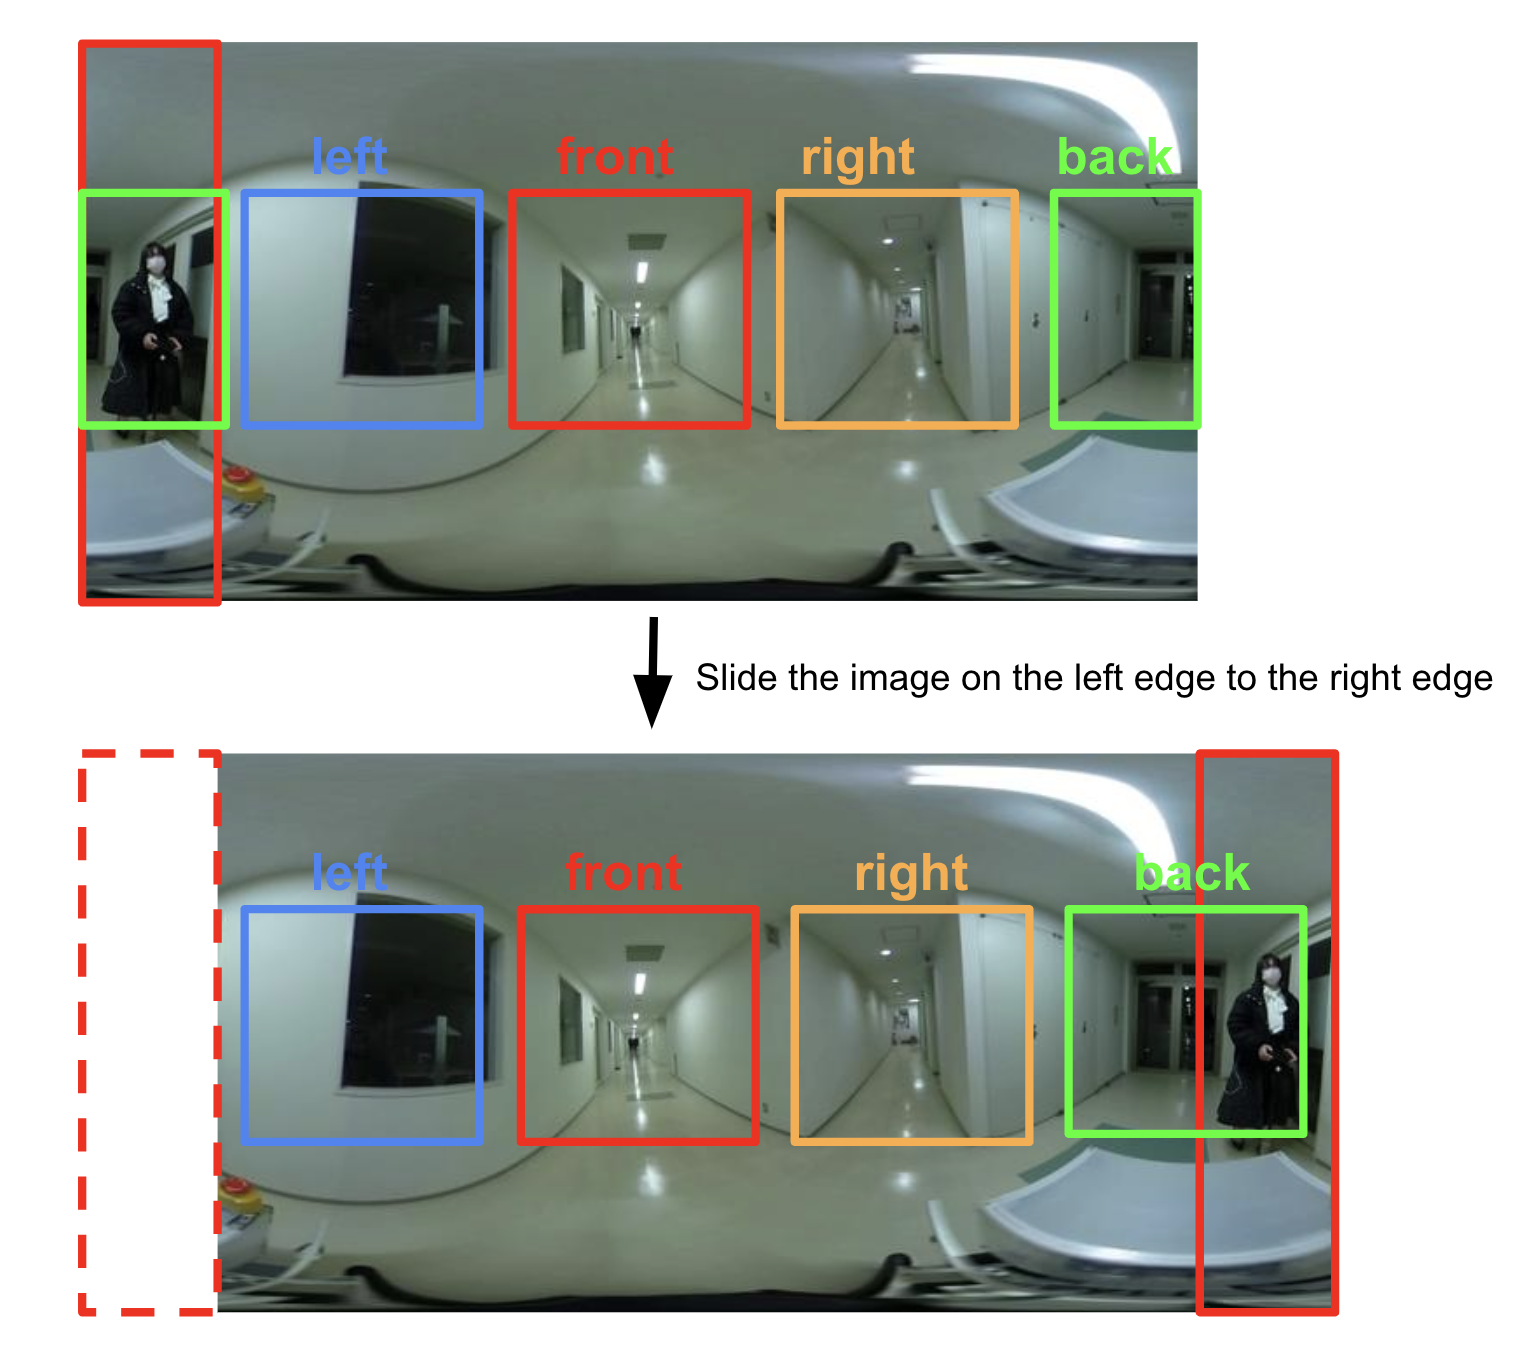
\includegraphics[width=10cm]{../images/image_proc2.png}
        %\caption{Preprocessing of spherical camera images.}
        %\label{figure::image_proc_fig}
        %\end{figure}